\section{An Audited Protocol (K1)}
\label{sec:protocol}

The protocol has six parts. Each exists because a specific comparison in our own history would otherwise have been misread. Appendix~\ref{app:audit} lists where we deviated from it. Fig.~\ref{fig:protocol} shows how the parts fit together.

\begin{figure*}[t]
\centering
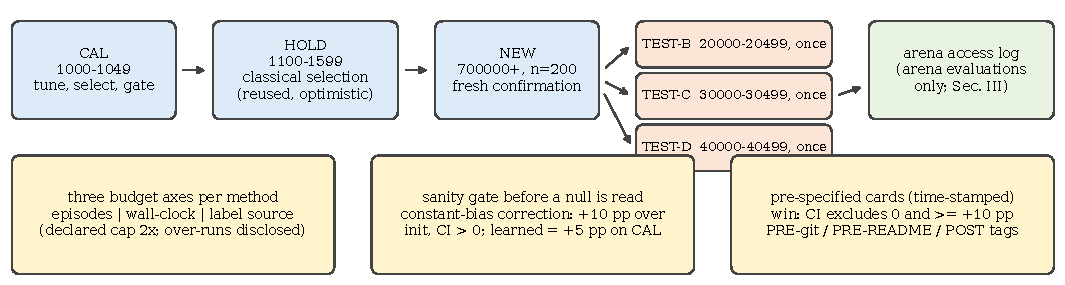
\includegraphics[width=\textwidth]{fig_protocol}
\caption{Protocol overview: seed-set roles (top) and the three rules that govern every comparison (bottom). The access log records arena evaluations on TEST seeds only.}
\label{fig:protocol}
\end{figure*}

\textbf{Extended classical tooling.} The classical side is not frozen at the textbook controller. It has a ladder of tuned variants (retuned gains, integral action, robust CMA-ES tuning, online system identification, and for whip an extended model class with 13 parameters; Section~\ref{sec:setup}). We call this tooling \emph{extended on the same footing} as the learner's, not equal on every axis: the classical side receives the generative parameter distribution as bounds and priors, and the learner receives it as simulated training data with labels.

\textbf{Three-axis budgets.} Every method reports episodes, wall-clock and label source, and the declared cap is 2$\times$ the classical episode budget. The learned side exceeded the cap in 4 of the 8 spikes of Appendix~\ref{app:budget}: it used 2.3$\times$ in the juggling PPO run, about 7$\times$ in the whip PPO sweep, 9--17$\times$ in the estimator duel and 3.2$\times$ in the idealised-whip re-run; in the other direction the classical tuning used about 7.7$\times$ the simulation steps of one RL policy in the first tracking study (Appendix~\ref{app:budget}). We report these ratios instead of equalising them.

\textbf{Pre-specified rules.} Hypotheses, metrics and decision rules are written in time-stamped, version-controlled cards (no external registry). A \emph{win} requires a paired bootstrap CI that excludes 0 and a gain of at least 10\% (tracking) or +10\pp\ (success rate); the +10\pp\ bar is our own choice and is not derived from a noise floor. Multiple tests inside one hypothesis family use Holm correction. Git order (rule committed before result) was verified for six early spikes (and for the headline rules of three more) and for the two locked-set runs of Section~\ref{sec:k3}; for ten spikes (01, 02, 03a, 04, 11a, 13b, 15b--15d, 16a) it cannot be shown because rule and result share a commit or the rule lived in a task prompt (Table~\ref{tab:audit}). No case was found in which git shows a rule committed after its result (Appendix~\ref{app:audit}). We therefore tag each result as pre-specified in git (\textbf{PRE-git}), pre-specified in a spike README only (\textbf{PRE-README}), or post hoc (\textbf{POST}). Because ``no win at +10\pp'' is not ``matched'', we add post hoc two one-sided tests (TOST) from the 90\% CI at $\pm10$ and $\pm5$\pp; only rows whose whole 90\% CI lies inside the margin are called equivalent. CIs and $p$-values are not corrected across spikes.

\textbf{Disjoint seed sets with roles.} Table~\ref{tab:seeds} lists the sets. Tuning and selection use CAL; HOLD selected the best classical baseline in two spikes and was then reused, so it is optimistic for the classical side; the locked sets TEST-B, TEST-C and TEST-D were each evaluated once.

\begin{table}[t]
\centering
\caption{Seed sets. ``Locked'' sets were used once for the evaluation named in the last column.}
\label{tab:seeds}
\small
\begin{tabular}{@{}p{0.9cm}p{2.6cm}rp{3.1cm}@{}}
\toprule
Set & Seeds & $n$ & Role \\ \midrule
CAL & 1000--1049; +2000--2149 in spikes 13a--15c & 50 (200) & tuning, selection \\
HOLD & 1100--1599 & 500 & classical selection; reused \\
TEST & 0--49 & 50 & older spikes; reused for juggling \\
TEST-B & 20000--20499 & 500 & locked, realistic whip (Sec.~\ref{sec:k2}) \\
TEST-C & 30000--30499 & 500 & locked, ladder (card v8) \\
TEST-D & 40000--40499 & 500 & locked, plan selection (card v9) \\
NEW & 700000+ & 200 & fresh confirmation \\
\bottomrule
\end{tabular}
\end{table}

\textbf{Sanity gate and learning check.} Before a learner's null is interpreted, the learner must learn a known-learnable correction: a constant torque bias injected after a probe, with a pass of +10\pp\ over its initialisation with a CI above 0. A learner counts as having \emph{learned} only if its CAL-selected checkpoint beats initialisation by at least 5\pp. The first gate passed marginally: with the exploration log-std $-1.5$ and 3M steps, PPO gained +10.2\pp\ [4.8, 15.6] on HOLD ($n{=}500$), best of 8 gate runs, 0.2\pp\ above the threshold, judged on $n{=}500$ instead of the pre-specified $n{=}200$; the zero-residual rule ($\le$40\%) was not met and SAC did not pass. The gate taught a lesson: the default exploration scale (log-std $-3.5$, 0.36\,Nm) gave $-3.0$\pp\ [$-8.5$, +2.5] and learned nothing, while $-2.0$ gave +7.8\pp\ [3.0, 12.8]. Later gates are single-seed shots (Appendix~\ref{app:budget}), so every RL null below reads ``not learned under this recipe'', never ``cannot learn''.

\textbf{Audit log.} Every arena evaluation on TEST seeds appends a line to a log, which has 111 lines. The log covers arena evaluations only: the TEST evaluations of the first five spikes ran outside it, so the line count is not the number of locked-set accesses and must not be quoted alone. The three locked sets of Table~\ref{tab:seeds} were each accessed once.
